\section{Introduction}



\section{Experimental Design}

This section describes the experimental design of the proposed field experiment.
In this experiment, participants will use a pseudonymous online platform
to deliberate on a policy issue.
The deliberation will take place asynchronously, over a period of several days.
At several times throughout the deliberation,
participants will complete a ranked-choice poll regarding the policy issue,
allowing the evolution of their preferences to be tracked over the course of the
experiment.
Depending on opportunity and necessity, multiple waves of deliberation may
be conducted, each with a distinct policy issue and set of participants.


\subsection{Deliberative Topic}
The policy issue chosen as the topic of deliberation is a crucial component
of the experiment.
The topic will be chosen carefully according to several criteria.
The chosen policy issue must be:
\begin{itemize}
\item Relevant to the experimental population;
\item Amenable to participants changing their preferences based on new information or reasoning;
\item Amenable to a predefined list of proposed solutions;
\item Sufficiently complex to have three or more proposed solutions;
\item Timely, but unlikely to be influenced by current events during the deliberation.
\end{itemize}
Examples of policy issues meeting these criteria include:
\begin{itemize}
\item ``Where should the use of electric scooters be permitted?''
\item ``Given the COVID-19 pandemic, how should schools in the US reopen in Fall 2021?''
\end{itemize}


\subsection{Participant Recruitment and Incentives}
Participants will be recruited using several methods.
Participants will be recruited individually through posts on web forums
relevant to the policy question (e.g., reddit, facebook groups)
and to relevant email lists.
Participant pools will also be utilized,
including lists of previous participants
who have expressed interest in future studies
and the UMSI Online Recruitment System for Economic Experiments.
Individual participants will also be recruited using promoted posts and
advertisements on Twitter, Facebook, etc.
Separately, participants may also be recruited through partnership with
community groups who wish to try network deliberation as part of an organizational
decision-making strategy.
The number of such collaborations will depend on the number of interested
partner organizations that have decisions amenable to network deliberation
over the course of the experiment.

In order to incentivize participation and to compensate participants fairly
for their time,
participants who complete the deliberation and pre/post-experiment surveys
will be compensated financially.
Participants will be paid a predetermined fixed amount in order to
minimize the effect of the compensation on their deliberative behavior and
expressed preferences.


\subsection{Experimental Protocol}

Before the deliberation period begins,
participants will complete a short demographic survey.
This survey will enable the identification of sample bias in age, gender, race,
and other demographic factors.

Participants will be randomly assigned to one of three treatment/control groups
at time of enrollment:
\begin{description}
\item[Control]{
The control group will engage in conventional single large group deliberation.
Posts and comments made by participants in the control group will be visible
to all others in the control group for the entire duration of the deliberation.}
\item[Network Deliberation (Efficient)]{
Participants in this treatment group will be divided into small
(4--5 participant) pods.
Posts and comments made by participants in this treatment group will only be
visible to others in their current pod.
All participants will be assigned to a new pod at the beginning of each round
of deliberation using the random-pod assignment method,
producing a structurally efficient communication network.}
\item[Network Deliberation (Inefficient)]{
Participants in this treatment group will be divided into small
(4--5 participant) pods.
Posts and comments made by participants in this treatment group will only be
visible to others in their current pod.
All participants will be assigned to a new pod at the beginning of each round
of deliberation using the long-path assignment method,
producing a structurally inefficient communication network.}
\end{description}

The deliberation period will be divided into a predetermined number of {\em rounds},
each lasting a fixed length of time.
Present plans are to divide the deliberation period into three stages of two days
each.
However, these numbers may be adjusted to ensure time timeline of the
deliberation is consistent with any constraints imposed by specific policy issues.
Before and after each stage, participants will be asked to rank the proposed
solutions to the policy question according to their individual preference.
During each round, participants will be shown a discussion prompt and will be
able to post a response to that prompt.
Example prompts are shown in Table \ref{tab:prompts}.
Participants will be able to view and comment on the posts of other participants
assigned to the same pod.
Participants will also be able to view posts and comments that were visible to them
in previous rounds, but will no longer be able to interact with or reply to
those posts and comments.

\begin{table}
\center
\label{tab:prompts}
\begin{tabular}{|p{0.3in}|p{3.6in}|}
\hline
Stage & Prompt \\
\hline
1 &
Which proposals do you prefer, and why?
If there are disagreements, try asking questions to understand the perspective
of others and to understand the causes of the disagreement.
\\
\hline
2 & In the previous round of discussion, what opinions and reasoning did you
observe in your group?
How much agreement was there?
Were there any disagreements or conflicts?
If so, what were the sources of conflict, and how might they be resolved?
\\
\hline
3 &
What seem to be the most popular opinions?
Do you agree with them?
Has your opinion changed over the course of the discussion?
\\
\hline
\end{tabular}
\caption{Example prompts for each round of deliberation.}
\end{table}

\section{Qualitative Analysis}
In addition to quantitative data,
qualitative data will also be collected in conjunction with
the deliberation experiment.
These data will be used to corroborate the results of quantitative
analysis and to achieve a richer understanding of individual participants'
experience of network deliberation,
as well as to as well as identify common themes that may provide
insight into the strengths and weaknesses of network deliberation.

The text of participants' posts and comments throughout the deliberation
will be kept for analysis.
This text can potentially be used to identify deliberative behaviors that
lead to changes in preferences.
Similarly, this text can be used to track the diffusion of specific keywords,
arguments, and influence through the communication network.

A subset of participants will be randomly selected to participate in
60-minute semi-structured interviews about their experience.
The interview script can be found in Appendix \ref{apx:interview}.
These interviewed will be transcribed and qualitatively coded using a
grounded theory approach.
The initial code book will be developed by open-coding pilot study transcripts
and an initial subset of interview transcripts.


\subsection{Network Topologies}
The minimum number of participants required is determined by a number of factors.
First, the long-path pod assignment method results in a minimum number of pods,
determined by the chosen parameters.
Specifically, the pod assignments for each round beyond the first are determined
by a unique prime number,
and the number of pods is a multiple of that prime.
For $T=3$ rounds, two primes are necessary and choosing the lowest two (2, 3)
yields the lowest minimum number of pods: 3.
For all pods to have at least 4 members, the minimum number of participants in
the long-path treatment is 12.

The two network deliberation treatments must also have meaningfully different
structural properties,
which also necessitates a minimum number of participants.
Structural differences between these two networks become more pronounced
with a greater number of participants.
While properties such as the broadcast time (see Chapter \ref{chap:abm})
and average geodesic length can be used to compare the structural efficiency of
two networks,
they encounter a problem for these particular networks
when there is a small number of rounds:
for many pairs of individuals, no path will exist.
In practical terms,
an idea proposed by one participant may not have a plausible
path to reach some of the other participants by the end of the deliberation,
even if that idea is repeatedly shared by all who encounter it.
As an alternative, a form of k-connectivty can be used to measure
structural efficiency.
The k-connectivity is simply the fraction of possible paths that exist.
In other words, if each participant broadcasts a message, and that message is
repeated by all who encounter it, what is the average fraction of participants
a broadcast will reach?
Figure \ref{fig:kcon} shows the k-connectivity as a function of number of
participants for both the long-path and random-pod deliberation networks.
While there is no clear threshold for the necessary number of participants,
choosing a k-connectivity of $0.5$ (half of possible paths exist) seems a
reasonable heuristic.
For the chosen parameters, 35 or more participants are necessary to produce
a random-pod network with $>0.5$ k-connectivity and
a long-path network with $<0.5$ k-connectivity.

Combining the above considerations,
an absolute minimum of 12 participants per treatment is necessary to conduct
a wave of the experiment,
and a minimum of about 35 participants per treatment group is necessary to
observe differences between the network deliberation treatment conditions.

\begin{figure}
\label{fig:kcon}
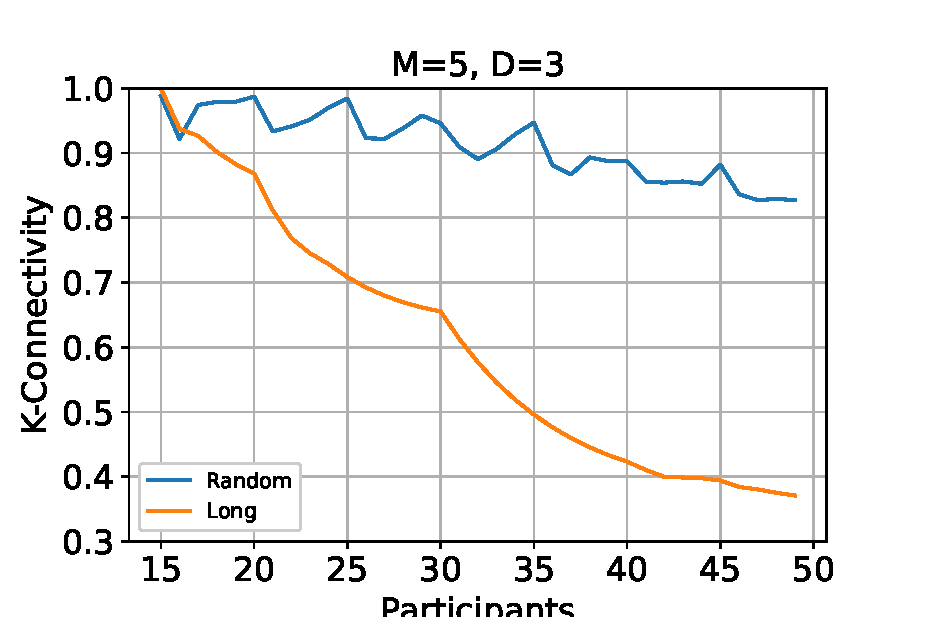
\includegraphics[width=5in]{fig/Experiment/fig-kcon.eps}
\caption{The k-connectivity of long-path and random-pod network deliberation
networks for $T=3$ stages and a pod size of $M=5$.}
\end{figure}

\subsection{Quantifying Preferences, Conflict, and Agreement}

\section{Study Software}

\section{Pilot Studies}
Several pilot studies have already been conducted:
one in a synchronous lab setting, and two using the asynchronous online
software.
In addition to providing an opportunity to test software,
these pilot studies have provided crucial information for developing a
feasible experimental design.

The initial pilot study was conducted on December 21, 2018,
before the custom online platform was developed.
In this pilot, NUMBER participants engaged in a synchronous 60-minute deliberation.
Participants sat at individual computer workstations, separated by dividers.
Participants discussed the following question:
``Where should the use of electric scooters be permitted?''
Participants were placed in a single treatment group, and divided into 4
pods of size 4--5.
These pods were reassigned using the random-pod method for a total of three
rounds.
The deliberation took place in chat rooms running the free and open-source
OTree online experiment software.

The second pilot took place after the initial development of the custom online
platform, from August 24, 2020 through August 32, 2020.

The third pilot took place from August 23, 2021 through August 29, 2021.

